\section{Numerical Experiments}\label{sect:numexp}
%
We now use Algorithm~\ref{alg:refSeries} to solve goal oriented inverse problems in a multi-model setting. We consider two kinds of multi-fidelity models, in a total of three experiments. In the first experiment, the high fidelity model is a convection-diffusion-reaction nonlinear model, and the low fidelity model is a linear convection-diffusion model. We examine how the localized error estimate is affected by changes in sensor placement and in the QoI region. In the second experiment, the high fidelity model uses an infinite dimensional (field) representation of the inferred parameter, while the low fidelity model uses a scalar representation. \red{The third experiment has the same setting as the first one, except a highly nonlinear version of the reaction term is considered, and showcases the robustness and computatioanal cost benefits of using the adaptive algorithm.}

%In all experiments, starting the simulation with the low fidelity model, we seek to add regions of high fidelity, until the estimated relative error in the target QoI is less than 1$\%$. 

%
\subsection{Error Estimate Localization}
%
Algorithm~\ref{alg:refSeries} does not require a particular method for localizing the error estimate. A na\"{i}ve approach would be to write the error estimate as a sum of integrals over elements and their boundaries, and calculate the error contribution by each element as the integral over that element. While perhaps simple to compute, this method results in non-zero error contributions from elements in which the high-fidelity model is already being used, making the error decomposition more difficult to interpret.

We instead use the alternative method described in \cite{vanOpstaletal15}, decomposing the error estimate into contributions from locally supported basis functions rather than elements. For convenience of notation in this section, we drop subscripts so that $\Psi=\Psi_{LF}$, $Q=Q_{HF}$, and $U=U_{HF}$; for our numerical experiments, we have $Q_{LF}\subset Q$ and $U_{LF}=U$. We note that the error estimate in Equation \ref{eq:finErrExp} can be equivalently written as
%
\begin{equation}
I(q_{HF},u_{HF})-I(q_{LF},u_{LF})=-\frac{1}{2}\mathcal{M}'_{HF,\Psi}(\Psi)(\Lambda)+\mathcal{L}'_{HF,\xi}(\xi_\Psi)(\chi_\Psi)+\mathcal{R}(e^3). \nonumber
\end{equation}
%
We consider a finite-dimensional \red{conforming} subspace $(Q^h\times U^h\times U^h)^3 \subset (Q\times U\times U)^3$ which contains the approximations $(\Lambda^h,\chi_\Psi^h)$. Define a basis $\Phi^h=\{(\varphi,\upvarphi)_i\}_{i\in I}$ consisting of locally supported functions such that span $\Phi^h=(Q^h\times U^h\times U^h)^3$; we can then write $(\Lambda^h,\chi_\Psi^h)=(\sum_{i\in I}\varphi_i\lambda_i,\sum_{i\in I}\upvarphi_i x_i)$. The error estimate
%
\begin{equation}
\epsilon = -\frac{1}{2}\mathcal{M}'_{HF,\Psi}(\Psi)(\Lambda)+\mathcal{L}'_{HF,\xi}(\xi_\Psi)(\chi_\Psi) \leq \sum_{i\in I} \varepsilon_i,
\end{equation}
%
where
%
\begin{equation}\label{eq:basisblame}
\varepsilon_i = \left| -\frac{1}{2}\mathcal{M}'_{HF,\Psi}(\Psi)(\lambda_i\varphi_i)+\mathcal{L}'_{HF,\xi}(\xi_\Psi)(x_i\upvarphi_i) \right|
\end{equation}
%
can be interpreted as the error contribution from the basis function $(\varphi,\upvarphi)_i$. The basis functions with the largest error contributions are flagged, and the elements in their support are refined. Using this method, elements in which the high-fidelity model is already being used are not interpreted as continuing to contribute to the error in the QoI and thus are not marked again for refinement. The only exceptions are elements near the interfaces between the low-fidelity and high-fidelity regions, as basis functions near the boundary may have their support divided between the two regions and thus have a nonzero error contribution. 
%
\subsection{Convection-Diffusion(-Reaction)} \label{sec:cdvcdr}
%
In this section, we consider a pair of models which differ in the physics included. In Section \ref{sec:cdvcdrSetup} we describe a baseline setup for a simple problem in 2D. Section \ref{sec:cdvcdrBaseRef} describes the results of applying Algorithm~\ref{alg:refSeries} to the baseline problem, and Section \ref{sec:qoivdata} describes the results of changing the placement of observations or the QoI region from the baseline.
%
%------------------------------------------------------------%
\subsubsection{Problem Setup} \label{sec:cdvcdrSetup}
%------------------------------------------------------------%
%
We consider a rectangular domain $\Omega(x_1,x_2)=[0,5]\times[0,1]$, where $x_1$ and $x_2$ are the spatial coordinates. The high-fidelity model is a single-species convection-diffusion-reaction equation with a nonlinear reaction term, described by,
%
\begin{subequations}
\label{eq:cdvcdrHF}
\begin{align}
k_d\nabla^2 u - \vec{V}\cdot\nabla u + k_ru^2 = f(q) \quad &\text{in } \Omega, \label{eq:cdvcdrHF_int} \\
u = 0 \quad &\text{on } \partial \Omega \label{eq:cdvcdrHF_bdry}
\end{align} 
\end{subequations}
%
where the state $u$ is the species concentration and $f(q)$ is a forcing field described by the parameters. We have a divergence-free parabolic-profile velocity field $\vec{V}(x_1,x_2) = (2x_2(1-x_2),0)$; the diffusion and reaction coefficients are $k_d = 0.1$ and $k_r = -42.0$, respectively. The low-fidelity model,
%
\begin{equation}
k_d\nabla^2 u - \vec{V}\cdot\nabla u = f(q)
\end{equation}
%
differs only in the removal of the reaction term. To form the mixed-fidelity models, we divide the domain into complementary subdomains, $\Omega_{HF}$ and $\Omega_{LF}$, where the high- and low-fidelity models are solved, respectively. The resulting mixed-fidelity models can be described by, 
%
\begin{equation}
k_d\nabla^2 u - \vec{V}\cdot\nabla u + k^{MF}_ru^2= f(q),
\end{equation}
%
where $k^{MF}_r$ is a piecewise-constant reaction coefficient,
%
\begin{equation}
k^{MF}_r=
\begin{cases}
-42.0 & \textrm{if }x\in\Omega_{HF} \\
0 & \textrm{if }x\in\Omega_{LF}.
\end{cases}
\end{equation}
%
The QoI we wish to calculate is the integral of the state,
%
\begin{equation}
I(q,u)=\int_{(x_1,x_2)\in \Omega_I} u \:\textrm{d}A,
\end{equation}
%
over a region $\Omega_I=[0.625,0.875]\times[0.375,0.625]$. 

The unknown parameters we wish to infer correspond to the forcing field, so that $f(q)=q$. For the low-fidelity model, the inverse problem is linear (the inferred parameters are linear in the observations). Observations consisting of the state at three points in the domain are artificially generated by running the high-fidelity model on a finer mesh with the true forcing field
%
\begin{equation}
f_{true}(x_1,x_2)=
\begin{cases}
1.0 & \textrm{if }(x_1,x_2)\in[0.125,0.375]\times[0.125,0.375] \\
0.8 & \textrm{if }(x_1,x_2)\in[2.375,2.625]\times[0.375,0.625] \\
0 & \textrm{otherwise}.
\end{cases}
\end{equation}
%
The locations of the observations and the region $\Omega_I$ over which the QoI is calculated are shown in Figure~\ref{fig:baseSetup}. Since the inverse problem is ill-posed, we use Tikhonov regularization~\cite{EngHanNeu00}; the regularization term is $\frac{\beta}{2}\int_\Omega \|\nabla f(q)\|_2^2\:\textrm{d}A$, where $\beta=10^{-5}$ is the regularization coefficient. 
%
\begin{figure}[h]
\centering
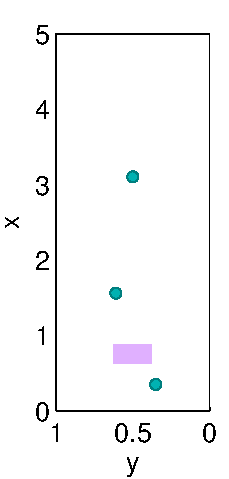
\includegraphics[width=0.8\textwidth]{baseSeries/setup_3_3.pdf}
\caption{Locations of the observations and the QoI region. \red{Aaaah spatial coordinates are not $x$ and $y$! ($y$ is one of the auxiliary variables...)}}
\label{fig:baseSetup}
\end{figure}
%

For the numerical simulations, we use the finite element method (FEM), employing a continuous Galerkin formulation with Lagrange elements. We use the \texttt{libMesh} library~\cite{libMeshPaper} for the FEM calculations. \red{The library offers easy calculation of adjoint systems, error estimates and subdomain restricted variables.}\footnote{But we don't use Libmesh's error estimates or restrict variables to subdomains...} The domain is discretized by a regular mesh of quadrilaterals, with 50 and 250 elements along the short and long boundaries, respectively, for a total of 12,500 elements, resulting in a total of 38,403 degrees of freedom. The diffusion coefficient is chosen so that the cell P\'{e}clet number never exceeds 0.1, and thus no stabilization is required.
%
%------------------------------------------------------------%
\subsubsection{Adaptive Model Refinement Results} \label{sec:cdvcdrBaseRef} 
%------------------------------------------------------------%
%
We now present the results for solving the inference problem using Algorithm~\ref{alg:refSeries}. Once the QoI error estimate is calculated using Equation~(\ref{eq:finErrExp}), the error estimate is then decomposed into local contributions, as described in Equation~(\ref{eq:basisblame}). At each iteration, based on this decomposition, we choose the basis functions with the largest error contributions until an additional 5\% of the elements has been marked for refinement. This is repeated until the estimated absolute relative error in the QoI, is less than $1\%$.

Figure~\ref{fig:baseRef} shows the local error contributions, as well as the subdomains where the low- and high-fidelity models are used, for the series of mixed-fidelity models thus generated. Each linear Langrange basis function's contribution is plotted at its nonzero node.
%
\begin{figure}[h!]
\captionsetup[subfigure]{justification=centering,aboveskip=-10pt}
\centering
  \begin{subfigure}[b]{\textwidth}
  \centering    
    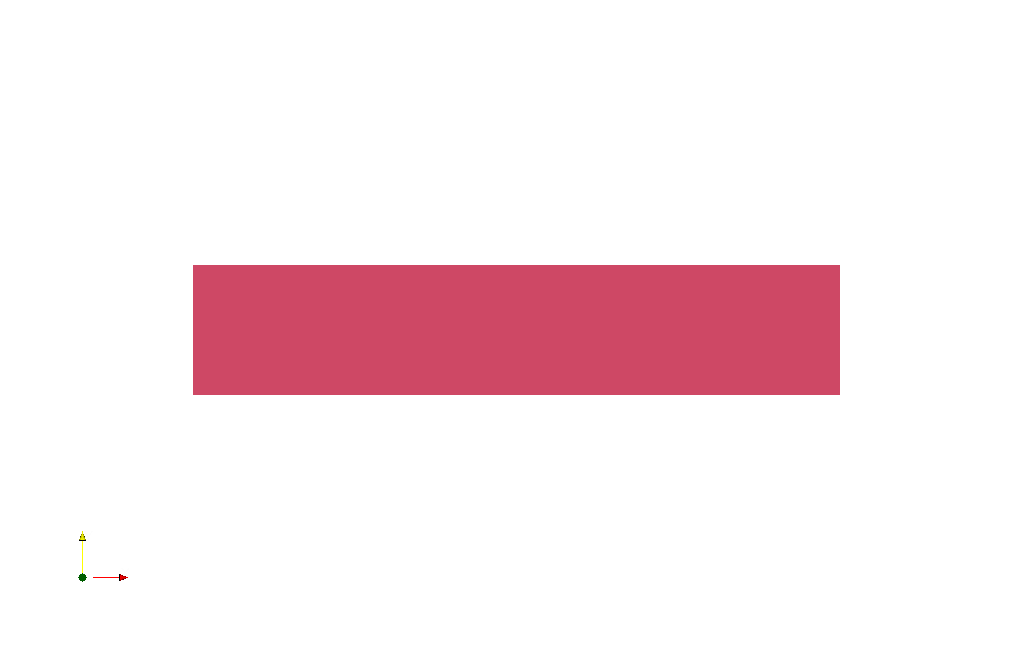
\includegraphics[width=0.48\textwidth]{baseSeries/cd_cdr_LF_divvy.png}
    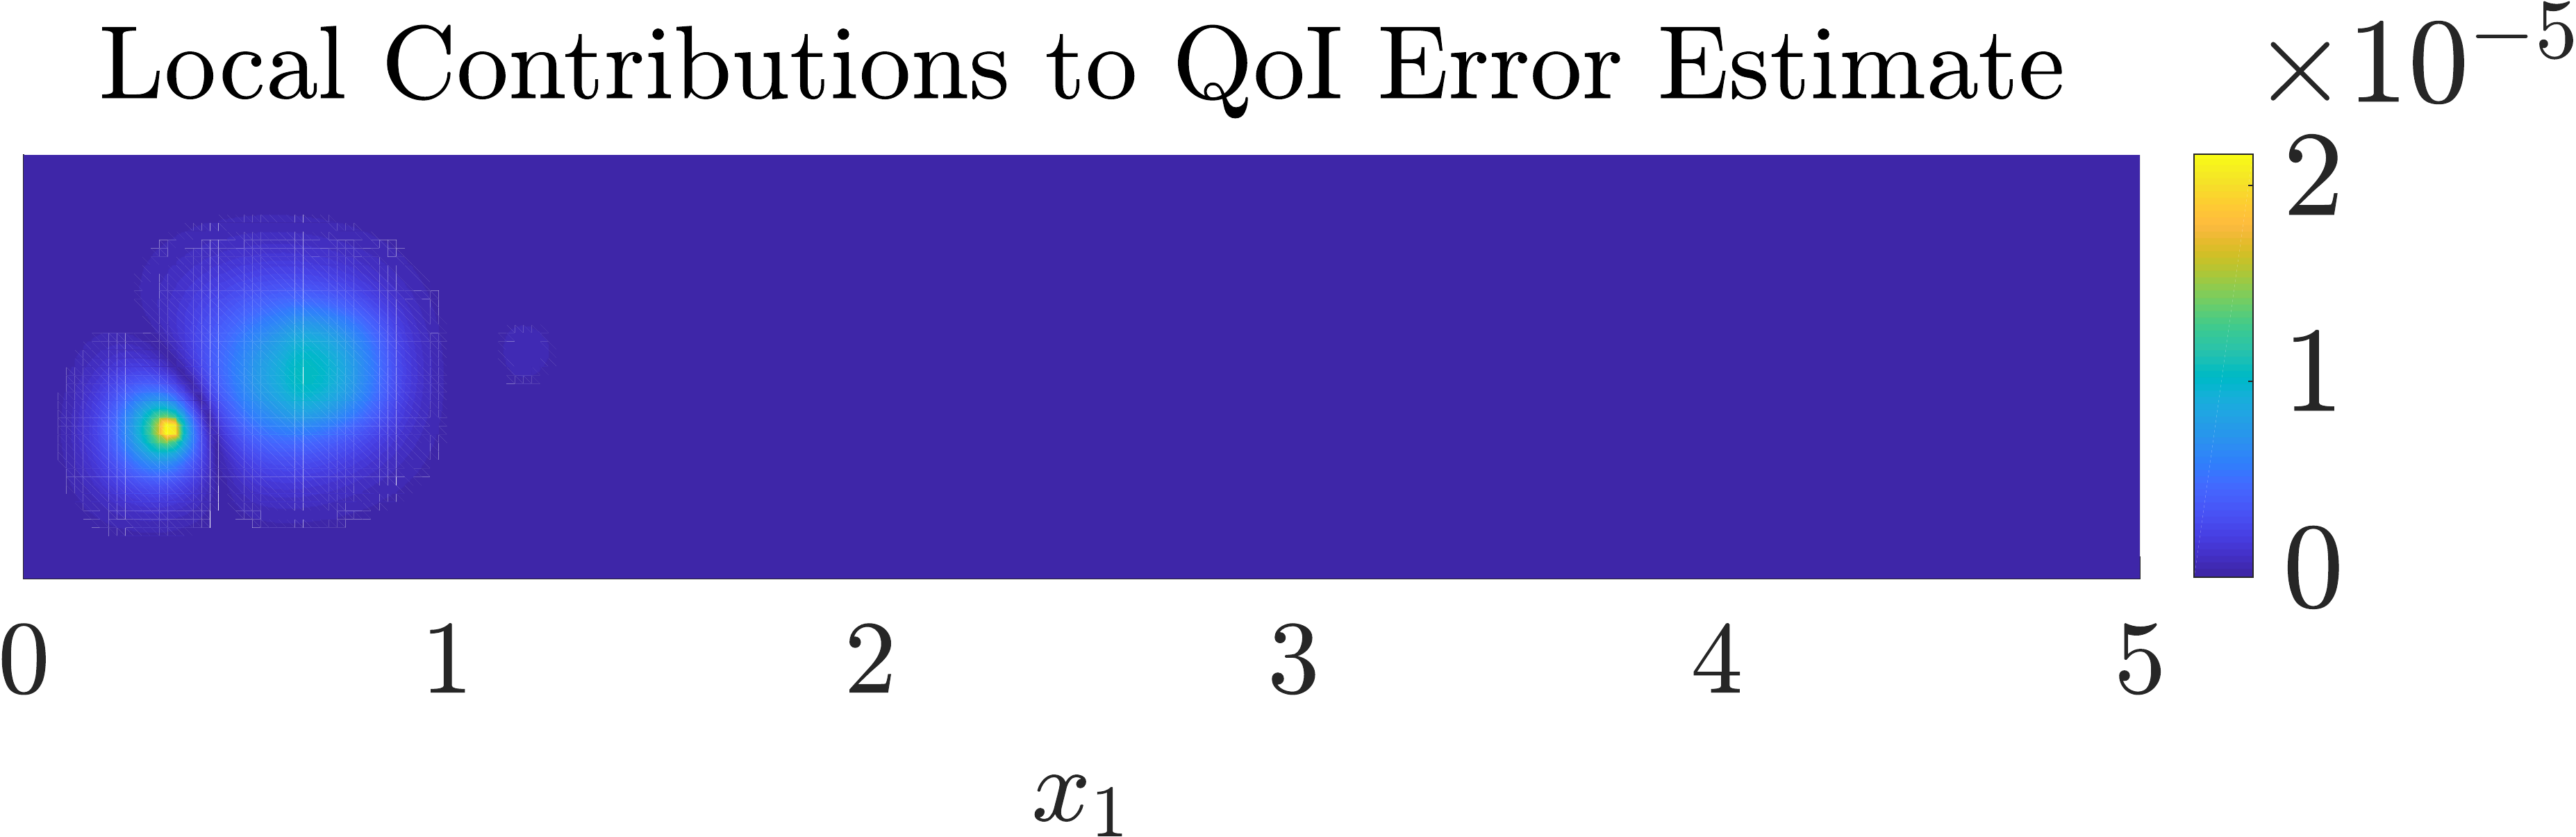
\includegraphics[width=0.51\textwidth]{baseSeries/err_breakdown_LF.png}
    \vspace{-0.5\baselineskip}
    \caption{MF$_0$ ($0\%$ HF)}
    \label{fig:baseRef0}
    \vspace{0.8\baselineskip}
  \end{subfigure}
	\begin{subfigure}[b]{\textwidth}
  \centering
    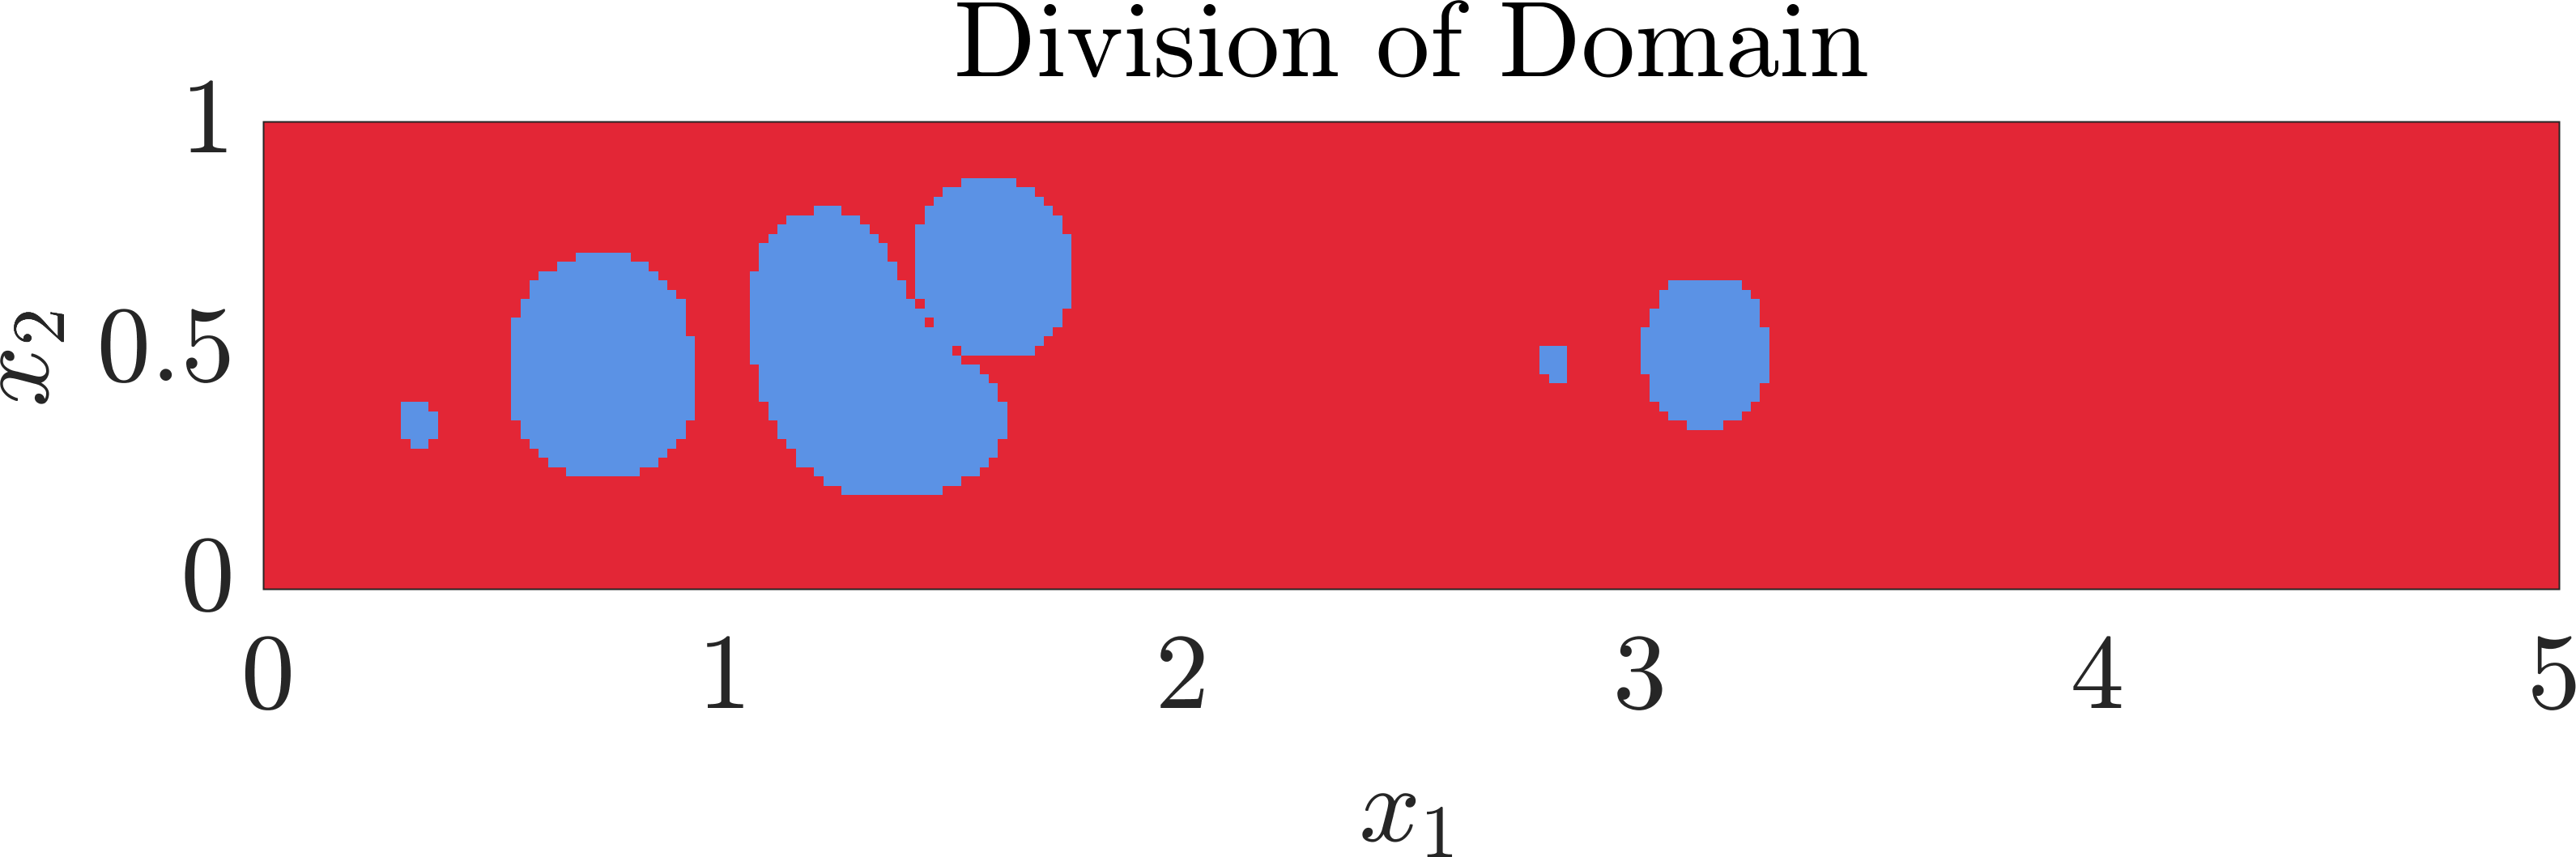
\includegraphics[width=0.48\textwidth]{baseSeries/cd_cdr_MF01_divvy.png}
    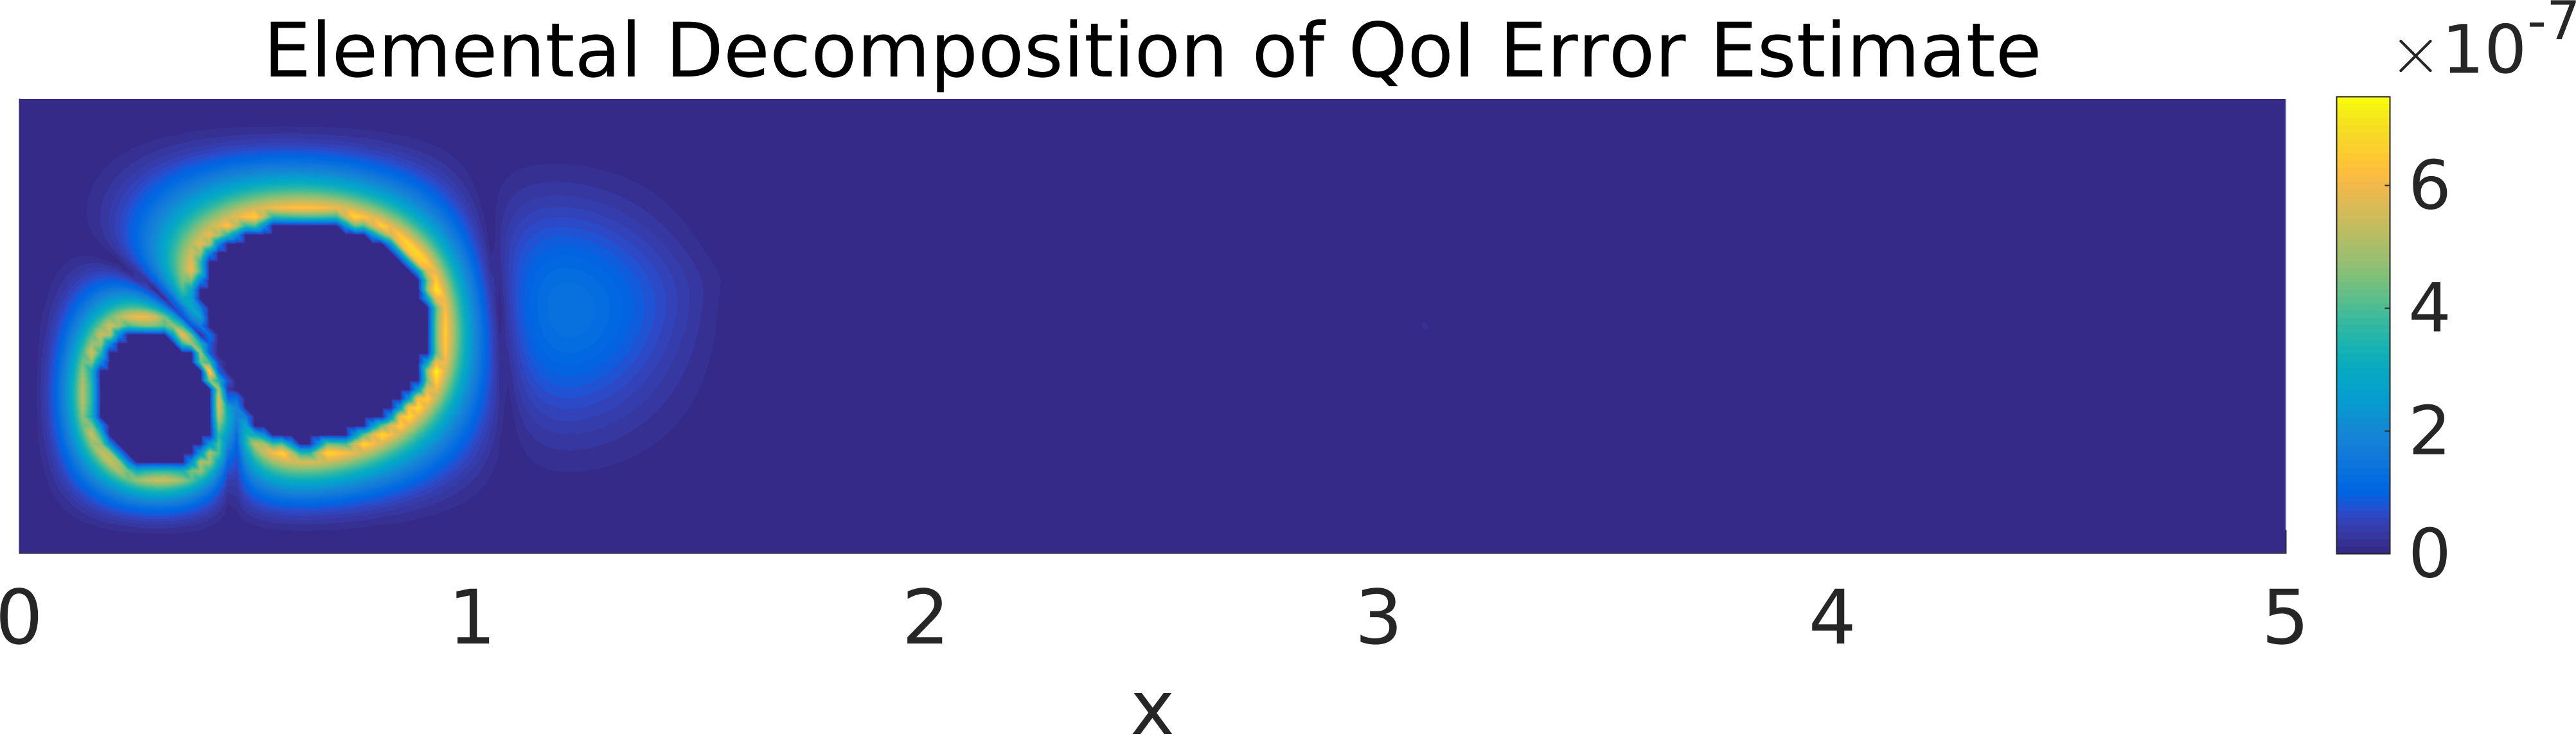
\includegraphics[width=0.51\textwidth]{baseSeries/err_breakdown_MF01.png}
    \vspace{-0.5\baselineskip}
    \caption{MF$_1$ ($5\%$ HF)}
    \vspace{0.8\baselineskip}
  \end{subfigure}
  \begin{subfigure}[b]{\textwidth}
  \centering
    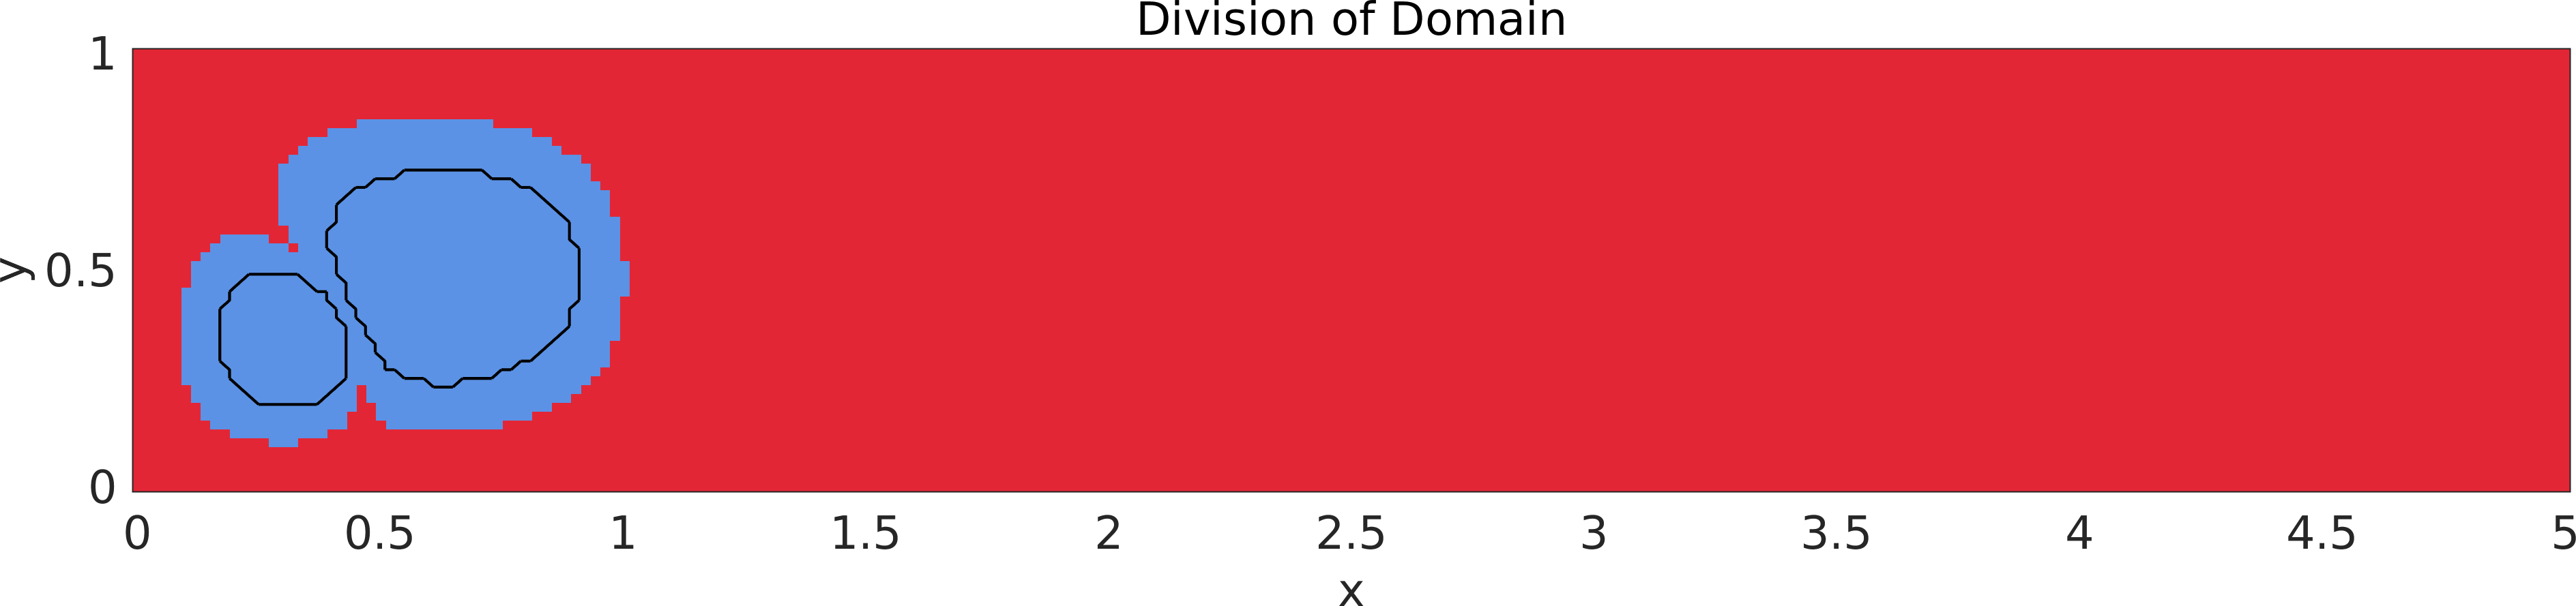
\includegraphics[width=0.48\textwidth]{baseSeries/cd_cdr_MF02_divvy.png}
    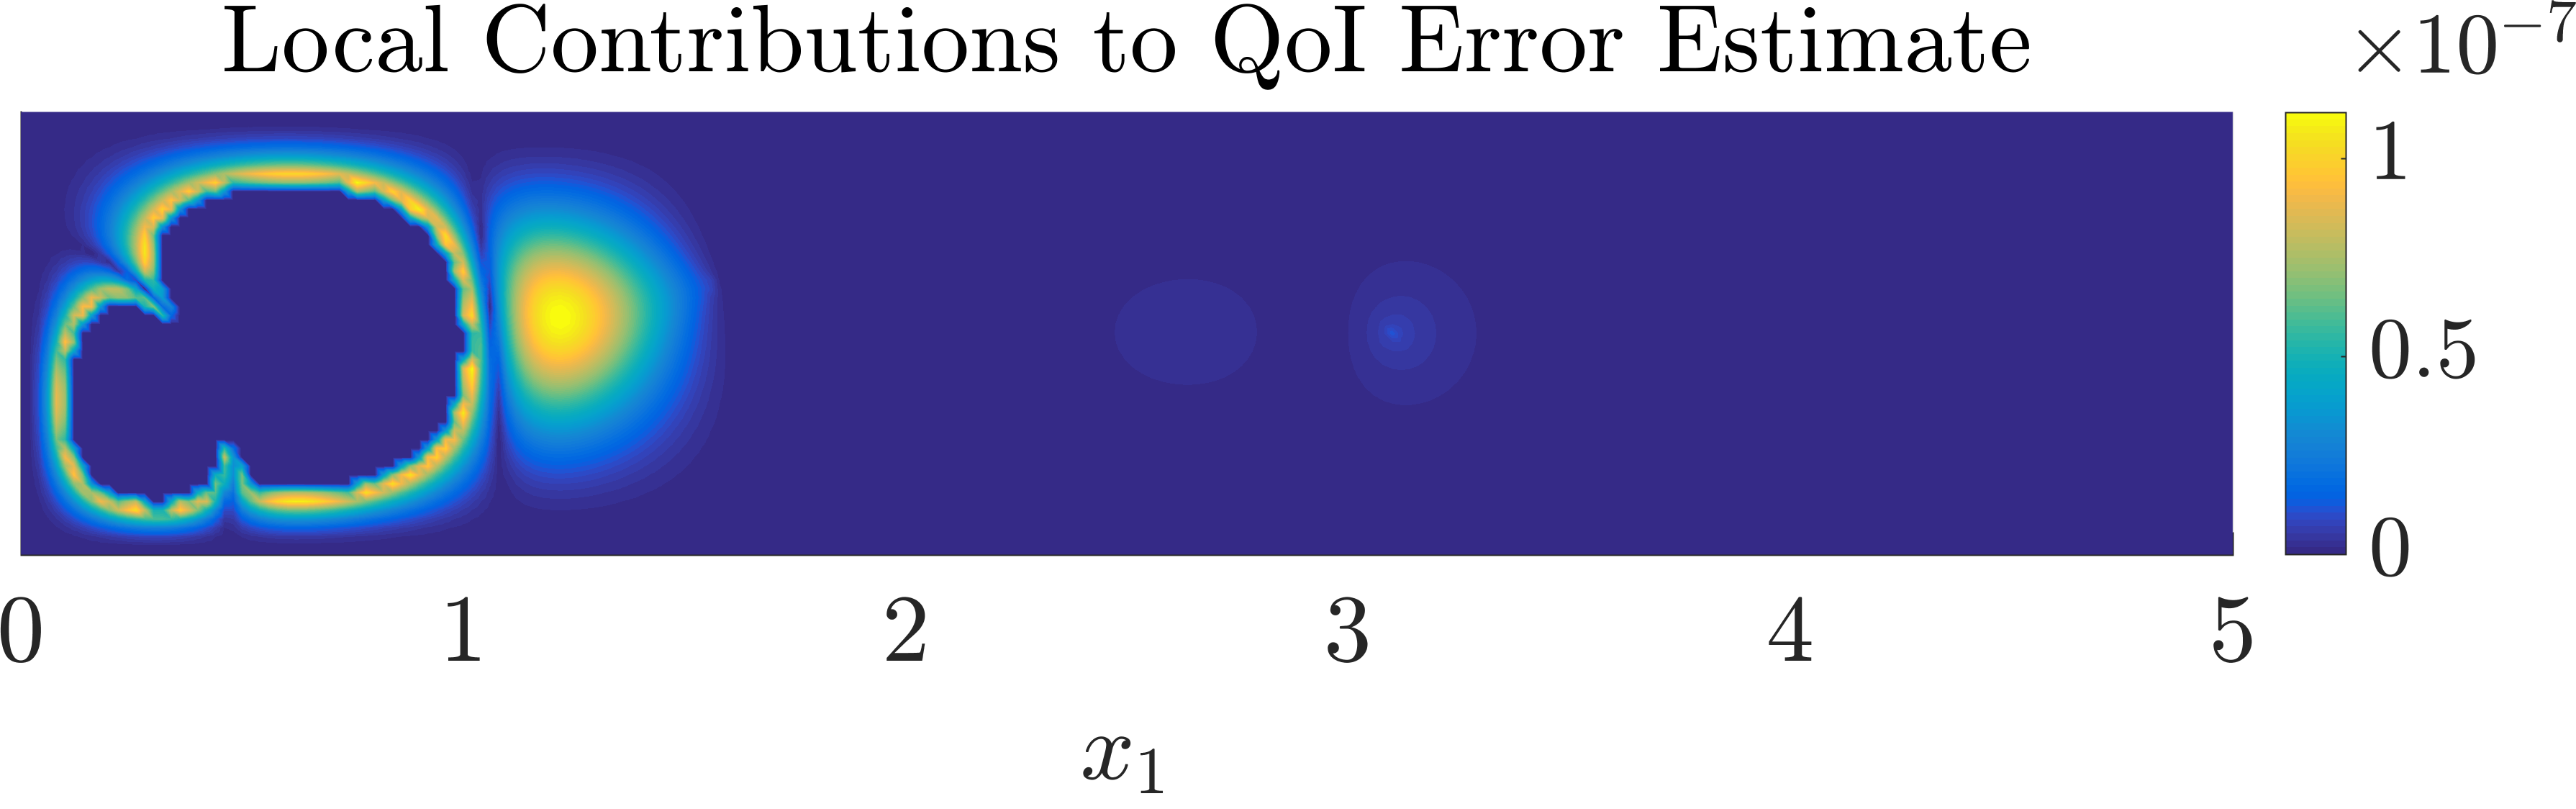
\includegraphics[width=0.51\textwidth]{baseSeries/err_breakdown_MF02.png}
    \vspace{-0.5\baselineskip}
    \caption{MF$_2$ ($10\%$ HF)}
    \vspace{0.8\baselineskip}
  \end{subfigure}
\caption{Local error contributions (right) and domain division (left; low-fidelity convection-diffusion model used in red portion, high-fidelity convection-diffusion-reaction model used in blue portion) for mixed-fidelity models.}
\label{fig:baseRef}
\end{figure}
%
Note that the error contribution of each basis function whose support is entirely within the high-fidelity regions is zero.

We see that the largest local error contribution is concentrated in the QoI region, and the data point closest to the QoI. In the first decomposition of the error (Figure~\ref{fig:baseRef0}), the region where the elemental error is maximum is the leftmost data point. Since the constraining model is an elliptic PDE, with a weak convection, information flow is localized, and is weakly convected from left to right. Therefore, for the calculation of the QoI, it is most important to refine the region near the leftmost data point, and the QoI region. After that, the error decomposition suggests refinement in regions upstream and around the middle data point, and then the rightmost data point.

Figure~\ref{fig:baseErr} shows the true and estimated absolute relative errors in the QoI for the various mixed-fidelity models generated by Algorithm~\ref{alg:refSeries}. In this case, we see that the QoI error of only $1\%$ is attained with a mixed-fidelity model where the high-fidelity model is used in only about $10\%$ of the domain. We note that there is no guarantee that either the error in the QoI or the relative error in the error estimate will decrease monotonically as more of the domain is refined.
%
\begin{figure}[h]
\centering
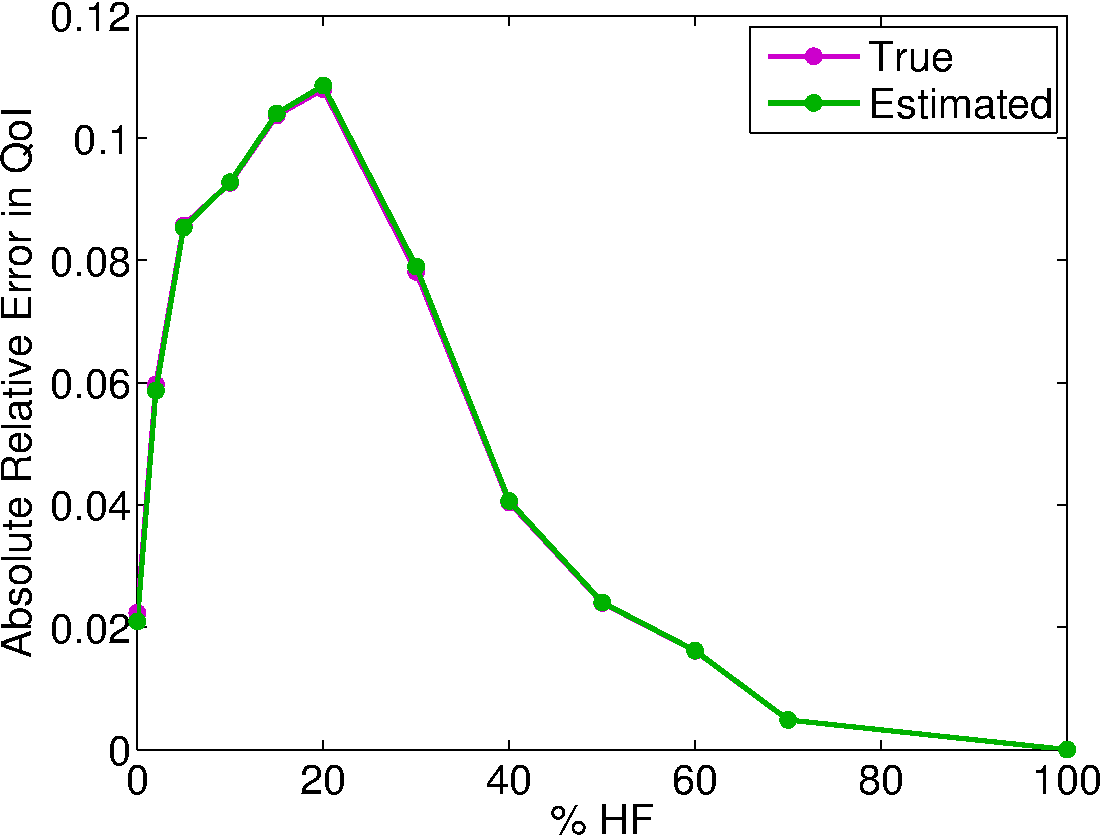
\includegraphics[width=0.7\textwidth]{baseSeries/err_est.pdf}
\caption{True and estimated absolute relative error in QoI, plotted as a function of the percentage area of the domain in which the high-fidelity convection-diffusion-reaction model is used.\red{does this even have enough points to warrant a graph? or would a table be better?}}
\label{fig:baseErr}
\end{figure}
%

%------------------------------------------------------------%
\subsubsection{Interaction of Observations and QoI} \label{sec:qoivdata}
%------------------------------------------------------------%
%
The error estimate decomposition (\ref{eq:basisblame}) suggests the use of the high-fidelity model in areas of the domain that are important to the interaction of the observations and QoI; the interaction of these two can be complex, and the areas suggested for refinement may be nonintuitive. To see this, we compare the error estimate decomposition for three sizes of the QoI region $\Omega_I$ given the same set of data points, and for three nested sets of data points given the same QoI region. For the sake of illustration, we make two refinement iterations for each combination of observations and QoI region, regardless of the magnitude of the relative error estimate. However, it was noticed that the number of iterations needed to achieve a given tolerance increased as the QoI region increased, but did not consistently increase or decrease with the number of data points.

The error decomposition for three increasingly large, nested QoI regions $\Omega_I$ given the same set of observations is shown in Figure \ref{fig:qoiStudy}. The bottom row gives the baseline case presented in Section~\ref{sec:cdvcdrBaseRef}, although here the basis functions with the largest $5\%$ of the error are choesn, so the proportion of additional refined elements in each iteration is slightly larger. Although refinement is still most important around the data point closest to $x_1=0$, as the QoI region expands the other two data points become more important in that the error decomposition suggests refinement around them earlier. As the QoI region expands, it is also more clearly noticeable that refinement is not equally important in all parts of the QoI region.

\begin{figure}
\captionsetup[subfigure]{justification=centering}
\centering
  \begin{subfigure}[t]{0.20\textwidth}
  \centering
    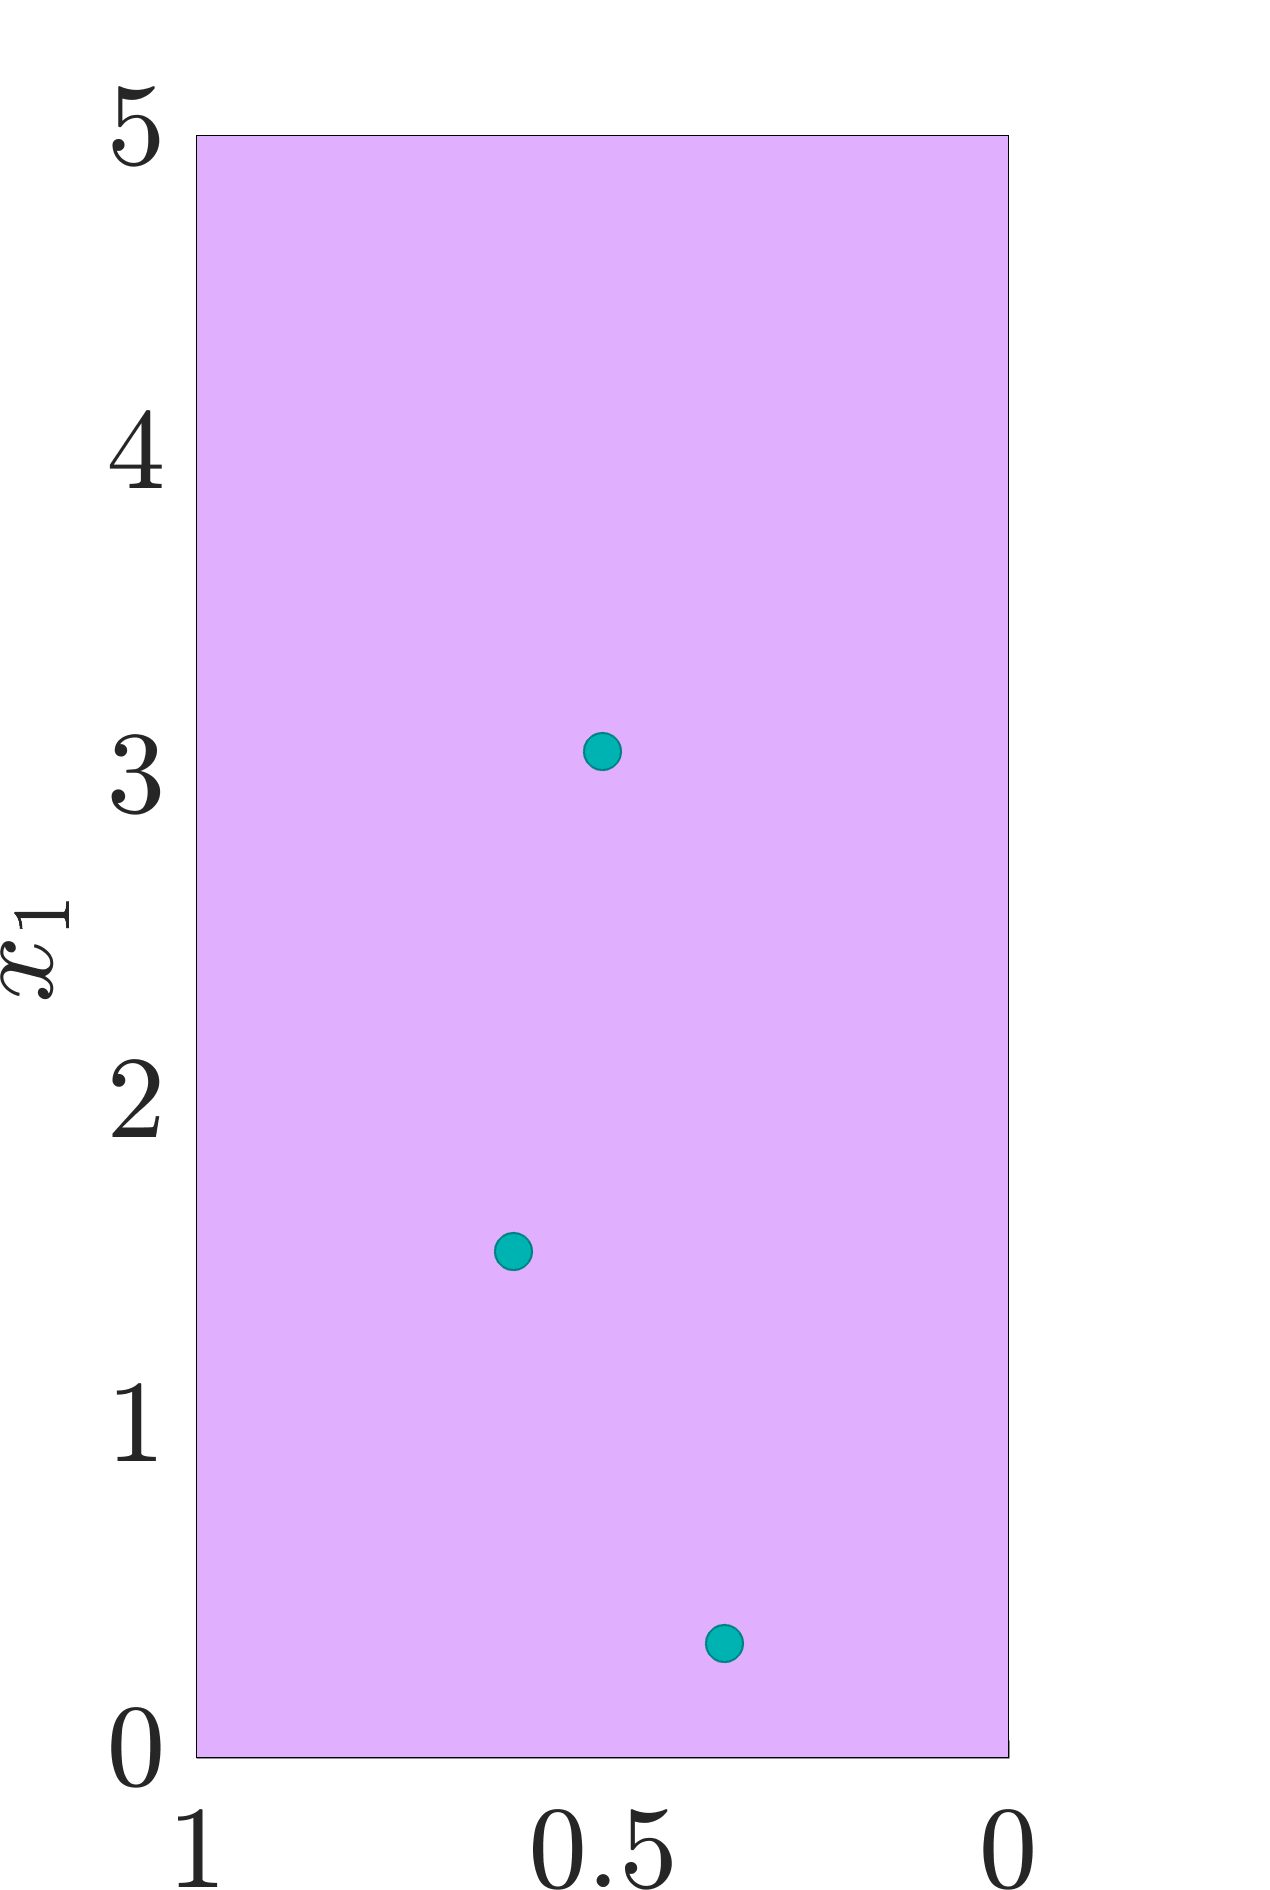
\includegraphics[width=\textwidth]{vs_qoi/qoi5_sens3/setup_5_3.png}
    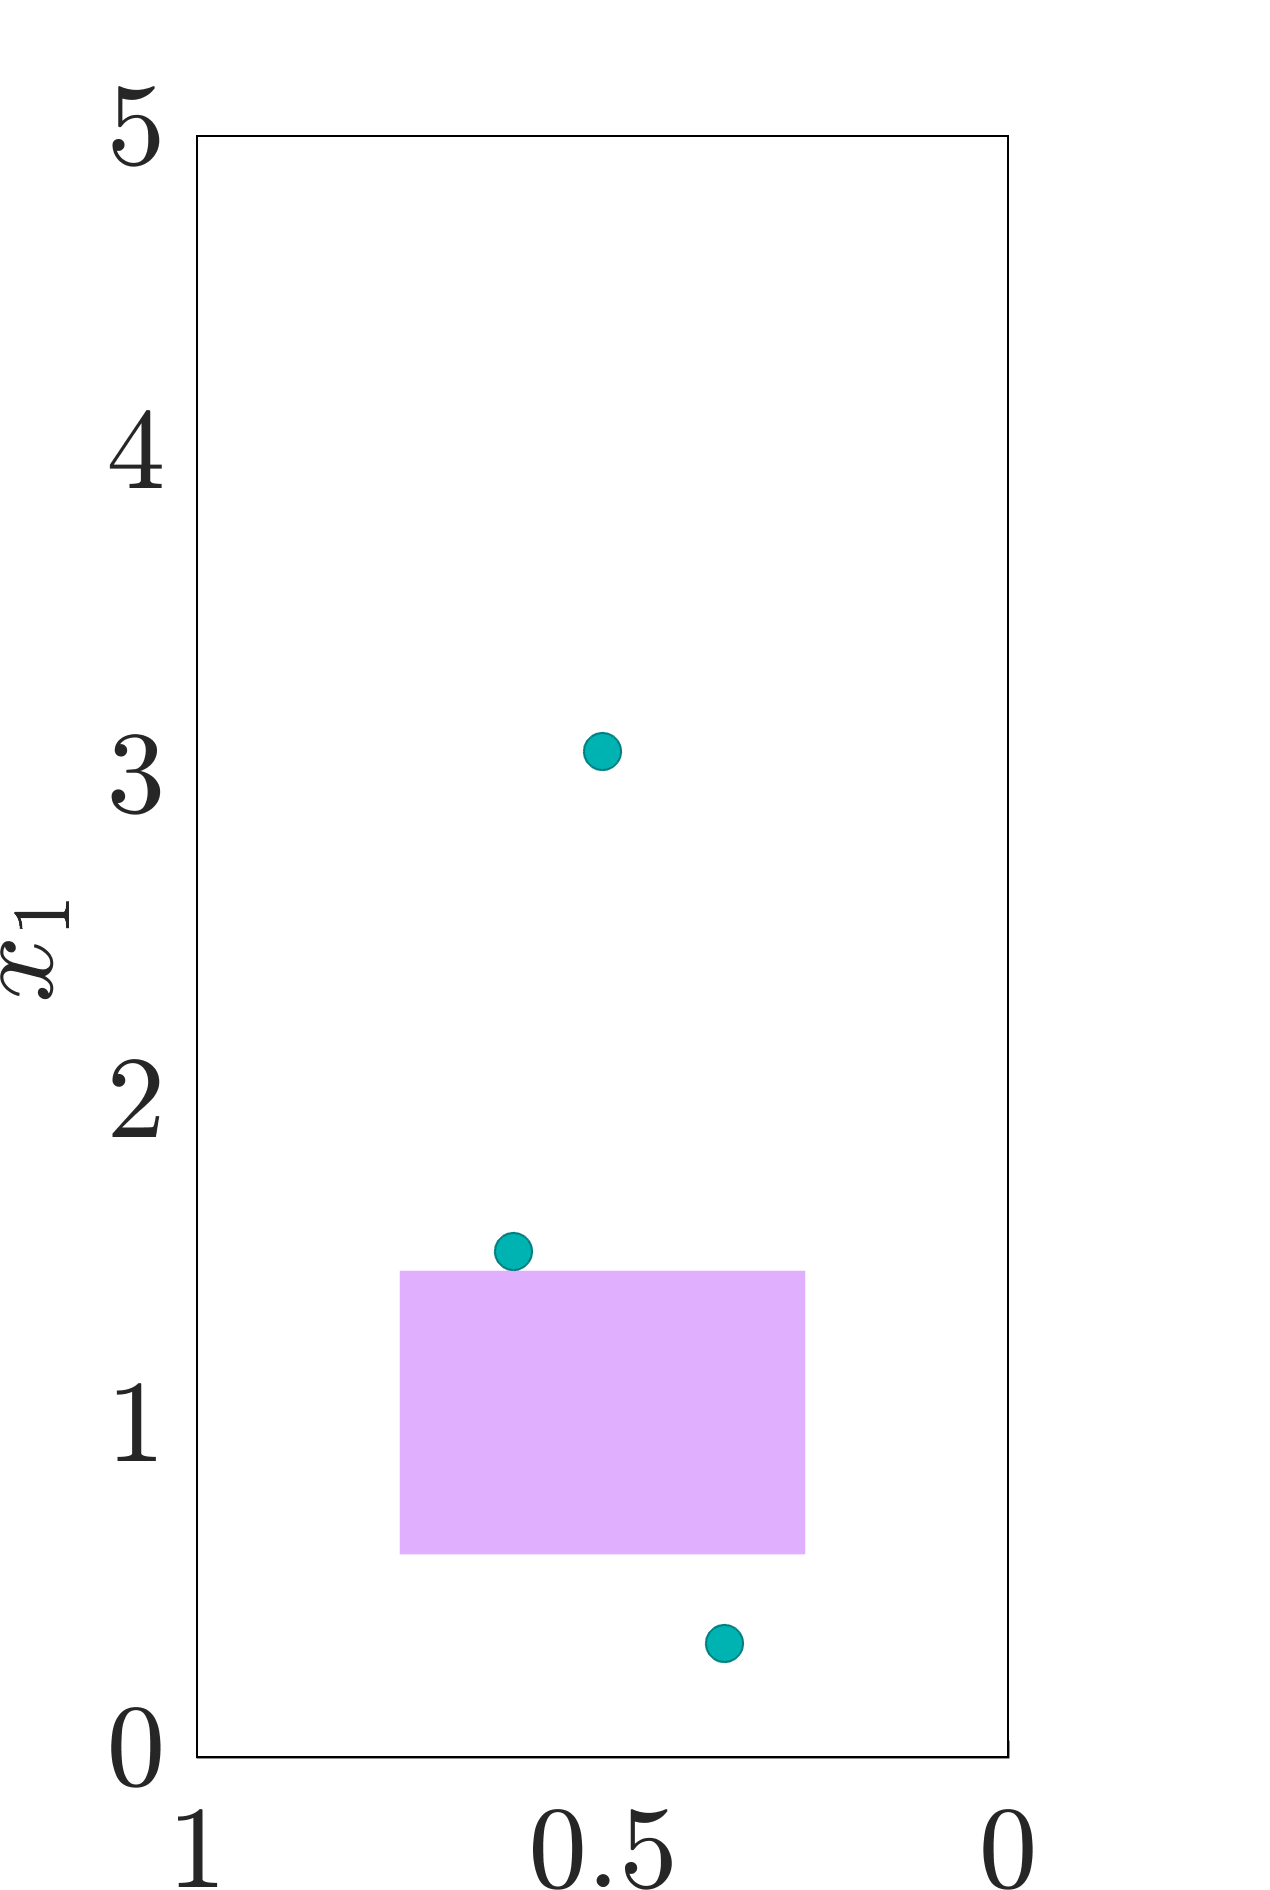
\includegraphics[width=\textwidth]{vs_qoi/qoi7_sens3/setup_7_3.png}
    \includegraphics[width=\textwidth]{vs_qoi/qoi3_sens3/setup_3_3.png}
    \caption{Locations of observations and QoI region $\Omega_I$}
    \label{subfig:obsSetup}
  \end{subfigure}
  \begin{subfigure}[t]{0.20\textwidth}
  \centering
    \includegraphics[width=\textwidth]{vs_qoi/qoi5_sens3/err_breakdown_0.png}
    \includegraphics[width=\textwidth]{vs_qoi/qoi7_sens3/err_breakdown_0.png}
    \includegraphics[width=\textwidth]{vs_qoi/qoi3_sens3/err_breakdown_0.png}
    \caption{MF$_0$ \\ ($0\%$ HF)}
    \label{subfig:obsLF}
  \end{subfigure}
  \begin{subfigure}[t]{0.20\textwidth}
  \centering
    \includegraphics[width=\textwidth]{vs_qoi/qoi5_sens3/err_breakdown_1.png}
    \includegraphics[width=\textwidth]{vs_qoi/qoi7_sens3/err_breakdown_1.png}
    \includegraphics[width=\textwidth]{vs_qoi/qoi3_sens3/err_breakdown_1.png}
    \caption{MF$_1$ \\ ($\sim5\%$ HF)}
  \end{subfigure}
  \begin{subfigure}[t]{0.20\textwidth}
  \centering
    \includegraphics[width=\textwidth]{vs_qoi/qoi5_sens3/err_breakdown_2.png}
    \includegraphics[width=\textwidth]{vs_qoi/qoi7_sens3/err_breakdown_2.png}
    \includegraphics[width=\textwidth]{vs_qoi/qoi3_sens3/err_breakdown_2.png}
    \caption{MF$_2$ \\ ($\sim10\%$ HF)}
    \label{subfig:obsMFlast}
  \end{subfigure}
  \caption{Compare the error estimate decomposition (\subref{subfig:obsLF}-\subref{subfig:obsMFlast}), given the same observations (teal points in (\subref{subfig:obsSetup})) and varying QoI region (purple box in (\subref{subfig:obsSetup})).}
  \label{fig:qoiStudy}
\end{figure}

The error decomposition for three increasing, nested sets of observations and the same QoI region $\Omega_I$ is shown in Figure \ref{fig:dataStudy}. Again, the bottom row gives the baseline case presented in Section~\ref{sec:cdvcdrBaseRef}, although here the basis functions with the largest $5\%$ of the error are choesn, so the proportion of additional refined elements in each iteration is slightly larger. Refinement appears to be consistently most important around the data point closest to $x_1=0$ and the QoI region. However, as more data points are added, it becomes no longer necessarily true that refinement becomes less important around data points as their distance from the QoI region increases. The data points also interact with each other in that placing data points in regions of previously relatively uniform error contribution tends to result in a new error decomposition that is positive or negative around the data points, with valleys of zero magnitude in between.

\begin{figure}
\captionsetup[subfigure]{justification=centering}
\centering
  \begin{subfigure}[t]{0.20\textwidth}
  \centering
    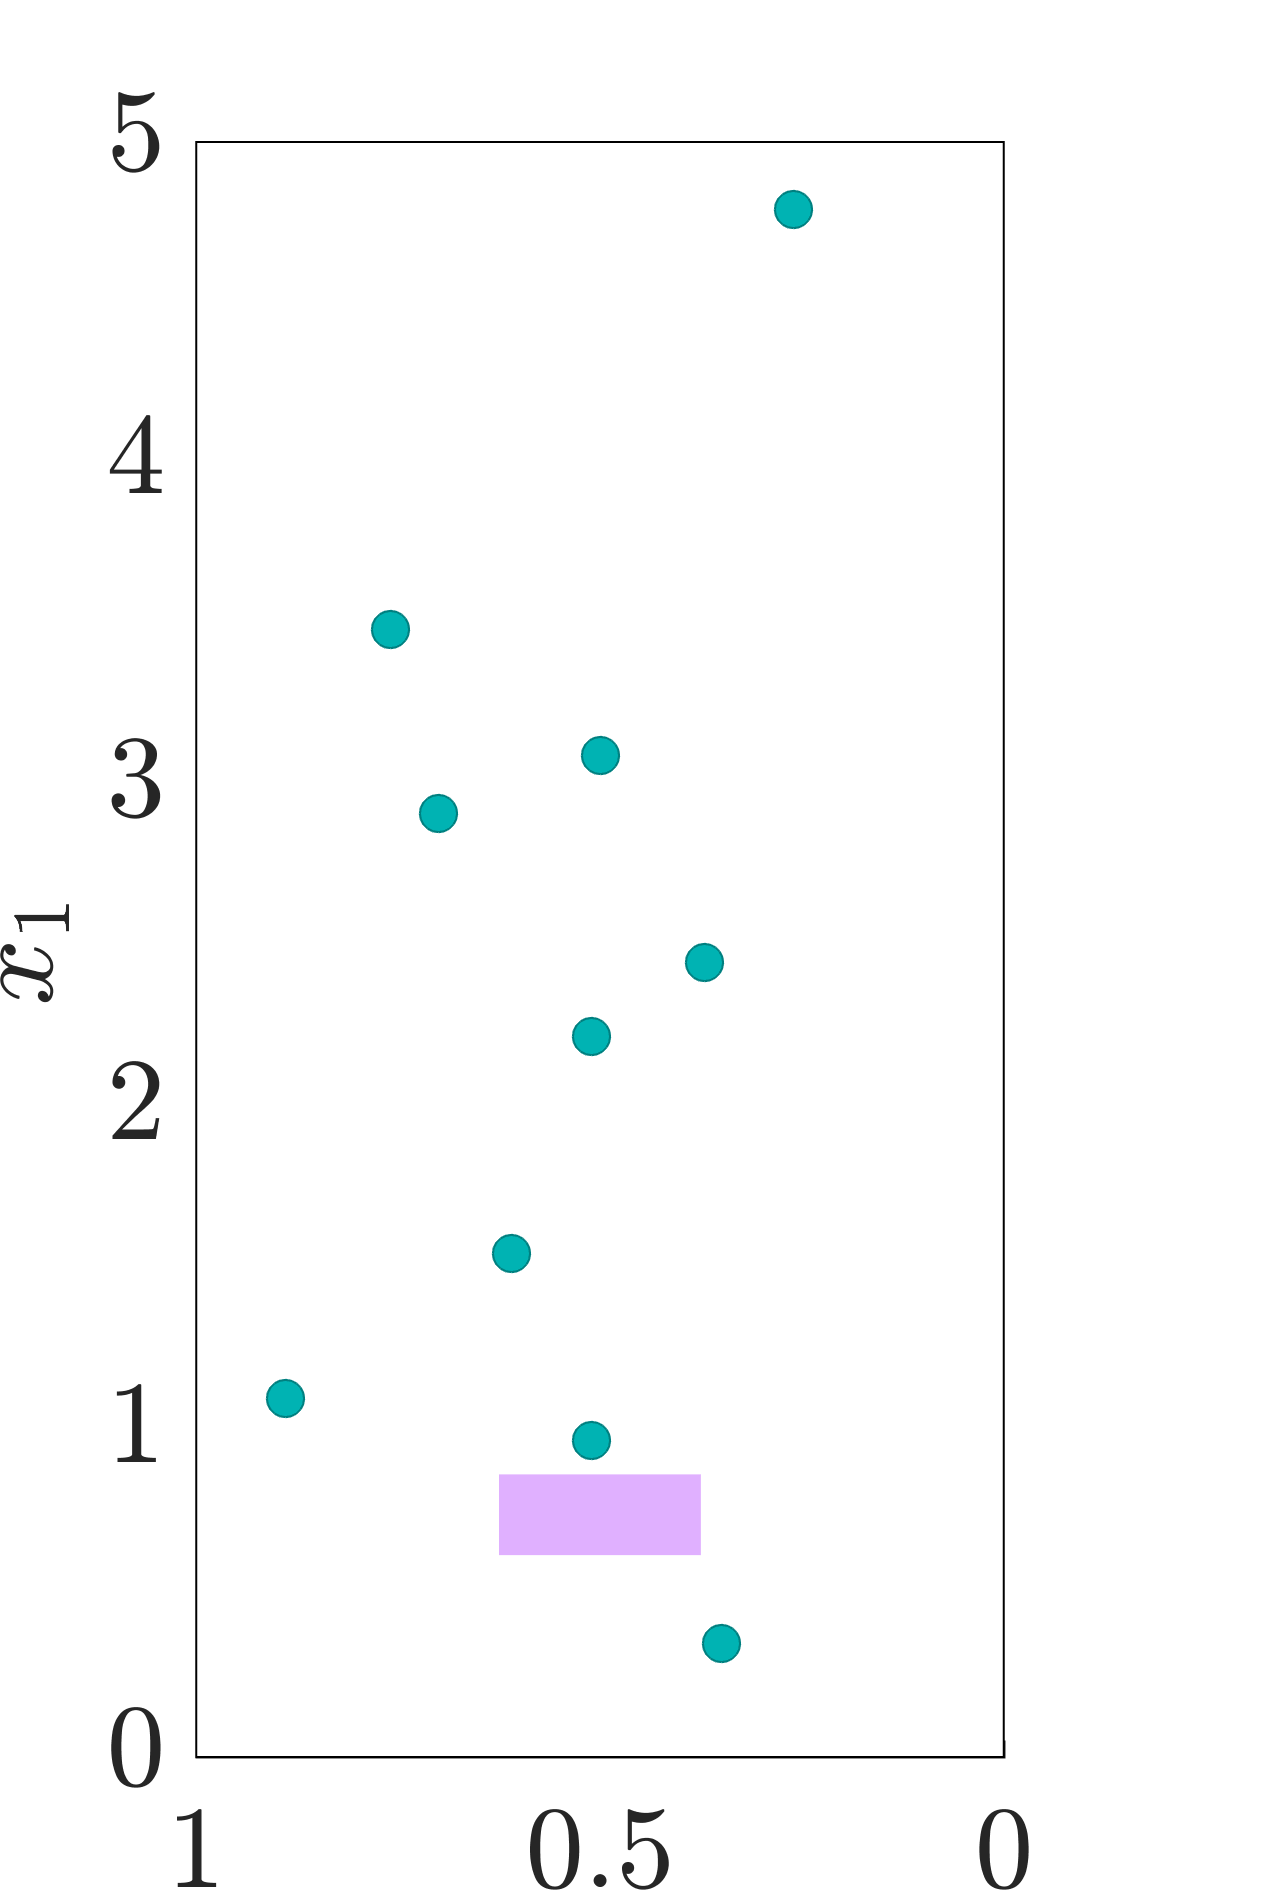
\includegraphics[width=\textwidth]{vs_data/qoi3_sens10/setup_3_10.png}
    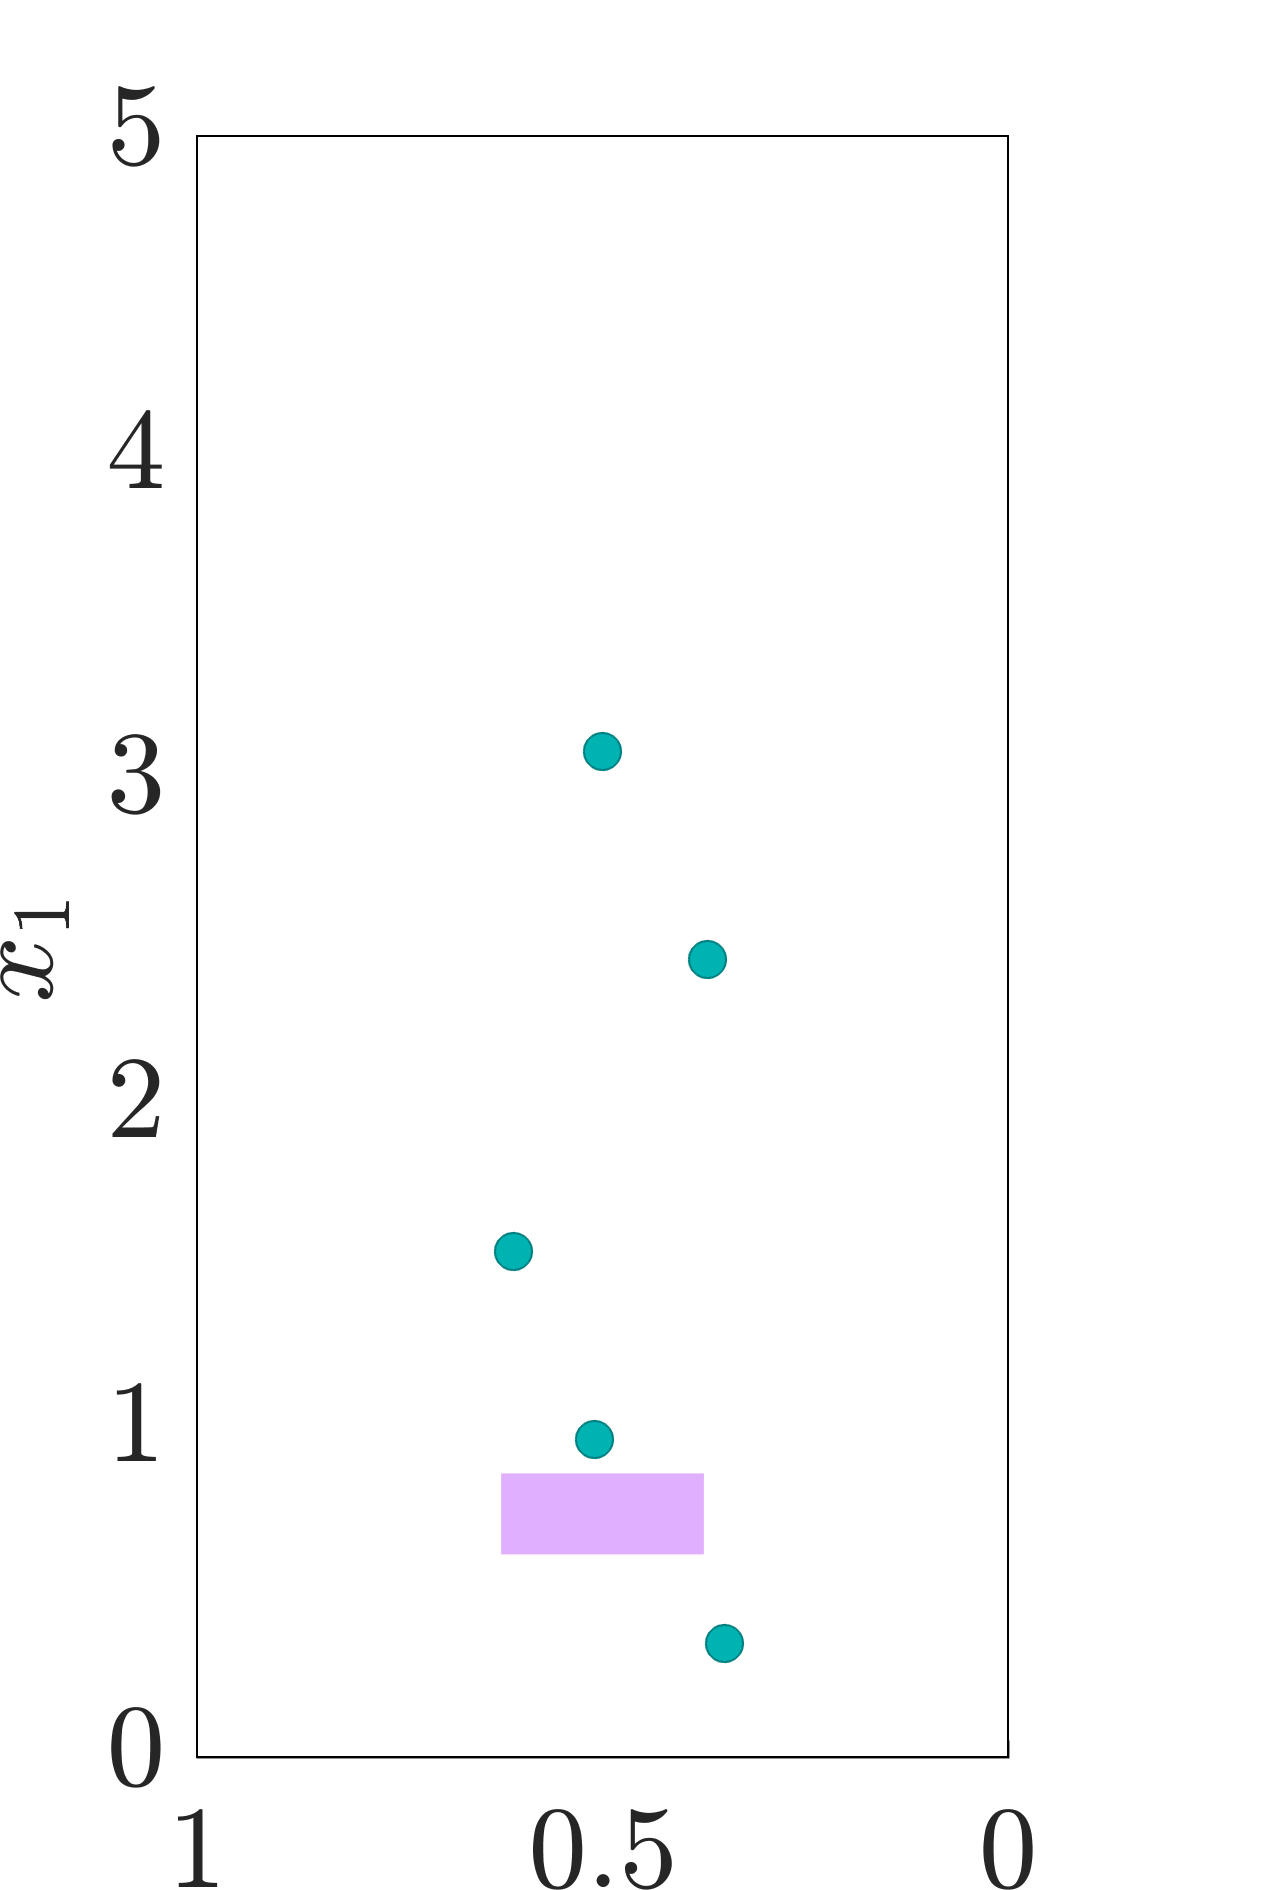
\includegraphics[width=\textwidth]{vs_data/qoi3_sens5/setup_3_5.png}
    \includegraphics[width=\textwidth]{vs_data/qoi3_sens3/setup_3_3.png}
    \caption{Locations of observations and QoI region $\Omega_I$}
    \label{subfig:obsSetup2}
  \end{subfigure}
  \begin{subfigure}[t]{0.20\textwidth}
  \centering
    \includegraphics[width=\textwidth]{vs_data/qoi3_sens10/err_breakdown_0.png}
    \includegraphics[width=\textwidth]{vs_data/qoi3_sens5/err_breakdown_0.png}
    \includegraphics[width=\textwidth]{vs_data/qoi3_sens3/err_breakdown_0.png}
    \caption{MF$_0$ \\ ($0\%$ HF)}
    \label{subfig:obsLF2}
  \end{subfigure}
  \begin{subfigure}[t]{0.20\textwidth}
  \centering
    \includegraphics[width=\textwidth]{vs_data/qoi3_sens10/err_breakdown_1.png}
    \includegraphics[width=\textwidth]{vs_data/qoi3_sens5/err_breakdown_1.png}
    \includegraphics[width=\textwidth]{vs_data/qoi3_sens3/err_breakdown_1.png}
    \caption{MF$_1$ \\ ($\sim5\%$ HF)}
  \end{subfigure}
  \begin{subfigure}[t]{0.20\textwidth}
  \centering
    \includegraphics[width=\textwidth]{vs_data/qoi3_sens10/err_breakdown_2.png}
    \includegraphics[width=\textwidth]{vs_data/qoi3_sens5/err_breakdown_2.png}
    \includegraphics[width=\textwidth]{vs_data/qoi3_sens3/err_breakdown_2.png}
    \caption{MF$_2$ \\ ($\sim10\%$ HF)}
    \label{subfig:obsMFlast2}
  \end{subfigure}
  \caption{Compare the error estimate decomposition (\subref{subfig:obsLF2}-\subref{subfig:obsMFlast2}), given the same QoI region (purple box in (\subref{subfig:obsSetup2})) and varying observations (teal points in (\subref{subfig:obsSetup2})).}
  \label{fig:dataStudy}
\end{figure}

%
\subsection{Constant vs Field Parameters}
%
\subsubsection{Problem Setup}
%
\subsubsection{Results}
%
%bigger steps in 3D problem because qoi region bigger?
\subsection{Convection-Diffusion(-Highly Nonlinear Reaction)}
%
\subsubsection{Results}
%
We consider the convection-diffusion-reaction term described in Section \ref{sec:cdvcdr}, with a reaction term $k_r=-616$ in the high-fidelity model. This reaction term is large enough that the Newton solver will not converge with a zero initial guess. We first solve the inverse problem with the low-fidelity model ($k_r=0$), and then use a simple continuation approach, using the solution at one value of $k_r$ as the initial guess for the next.\footnote{not arclength continuation, which is more difficult to implement, though libMesh appears to have a class for such continuation, which we can use if this seems like a viable direction} We increase the reaction term in increments of $\Delta k_r=100$, and halve the increment each time the step is too large (Newton solver does not converge at the next $k_r$ value). From $k_r=0$ to $k_r=-616$, this results in 9 continuation steps being taken.
%
\subsubsection{Computational Complexity}
%
We compare the complexity of Algorithm~\ref{alg:refSeries} and the continuation method for the high fidelity problem, in the context of the analysis developed in section~\ref{sect:alg_complexity}. For the high fidelity problem, with  with 9 continuation steps, we have $\sum\limits_{i=1}^{C} K_i=30$. 
 
With Gaussian elimination chosen as the linear solver, this gives us $T < 3$, i.e.\ a budget of 2 adaptive steps. Using Algorithm~\ref{alg:refSeries} with 2 refinement steps, and only $10\%$ of the domain refined to use the high-fidelity model, the estimated relative error is $<1\%$. Indeed, the ratio $\frac{C_{MF}}{C_{HF}}$ was $\frac{24}{30}$, indicating about $20\%$ reduction in computational cost, with the worst case linear solver used. 

In other words, on using Algorithm~\ref{alg:refSeries} for a highly nonlinear problem, even with the worst case linear solver, one can get to $<1\%$ error in the QoI, with a $20\%$ reduction in computational cost, while avoiding any need for continuation to handle nonlinearities. 
